% !TEX root = main-crime.tex

\section{Feature Extraction}
\label{ch2-sec:feature}

%As discussed in Section~\ref{sec:overview}, there are three types of features used in inference model. 
In this section, we will discuss the details of features used in our method. The two types of new features we use are extracted from Point-Of-Interest data and taxi flow data. Below we describe the datasets used to construct features and the characteristics of these features.

\begin{figure*}[t]
\centering
\subfigure[Total population]{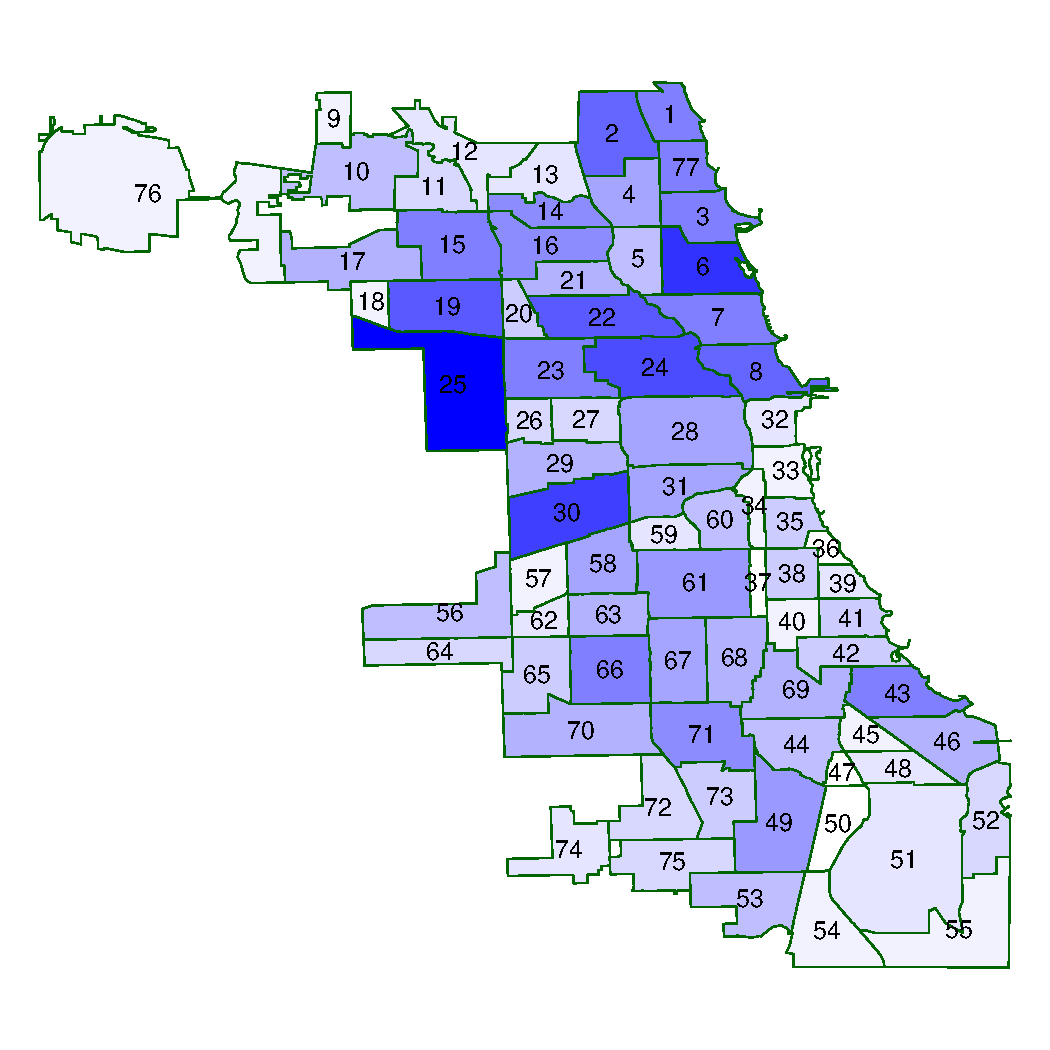
\includegraphics[width=0.45\textwidth]{fig/demo-f1.pdf}}
%\subfigure[Population density]{\includegraphics[width=0.22\textwidth]{fig/demo-f2.pdf}}
\subfigure[Poverty index]{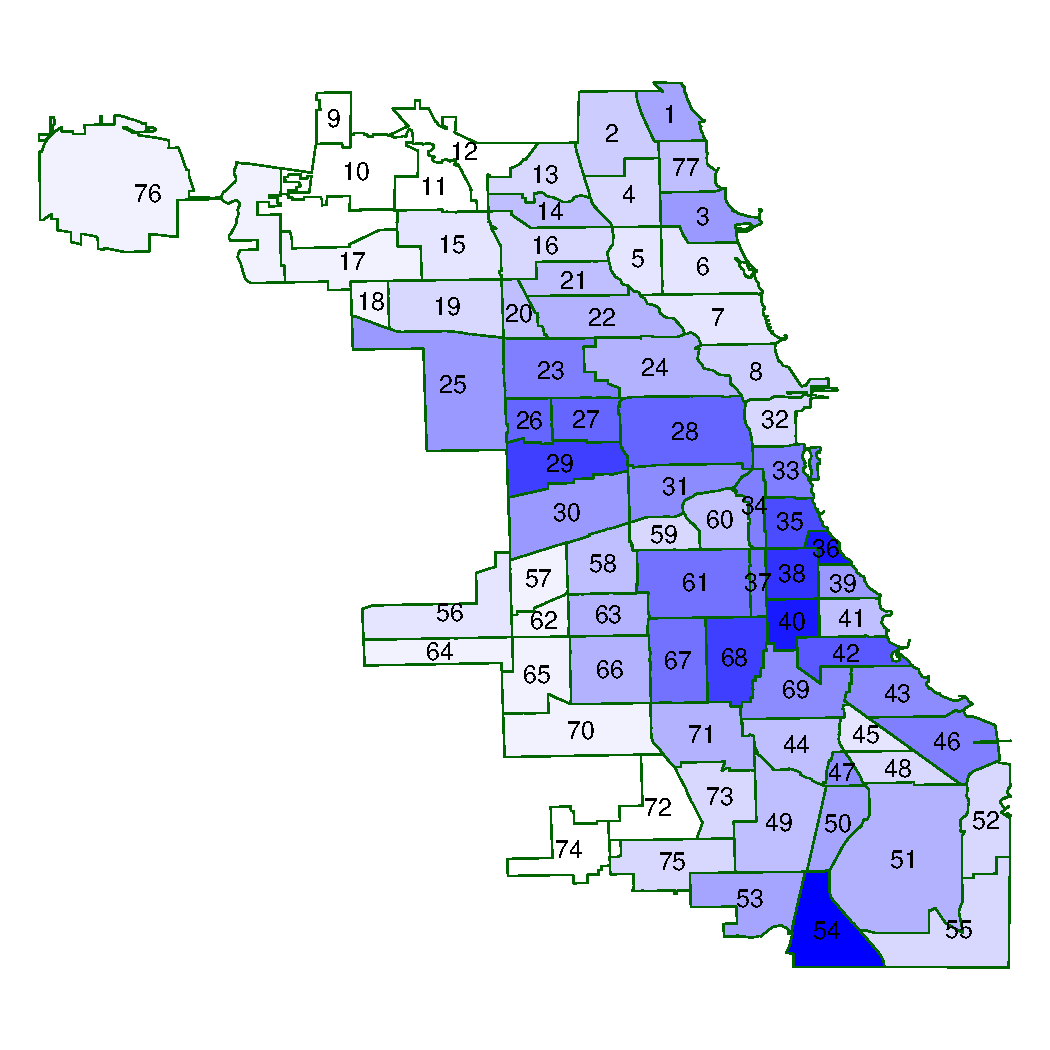
\includegraphics[width=0.45\textwidth]{fig/demo-f3.pdf}}
\subfigure[Disadvantage index]{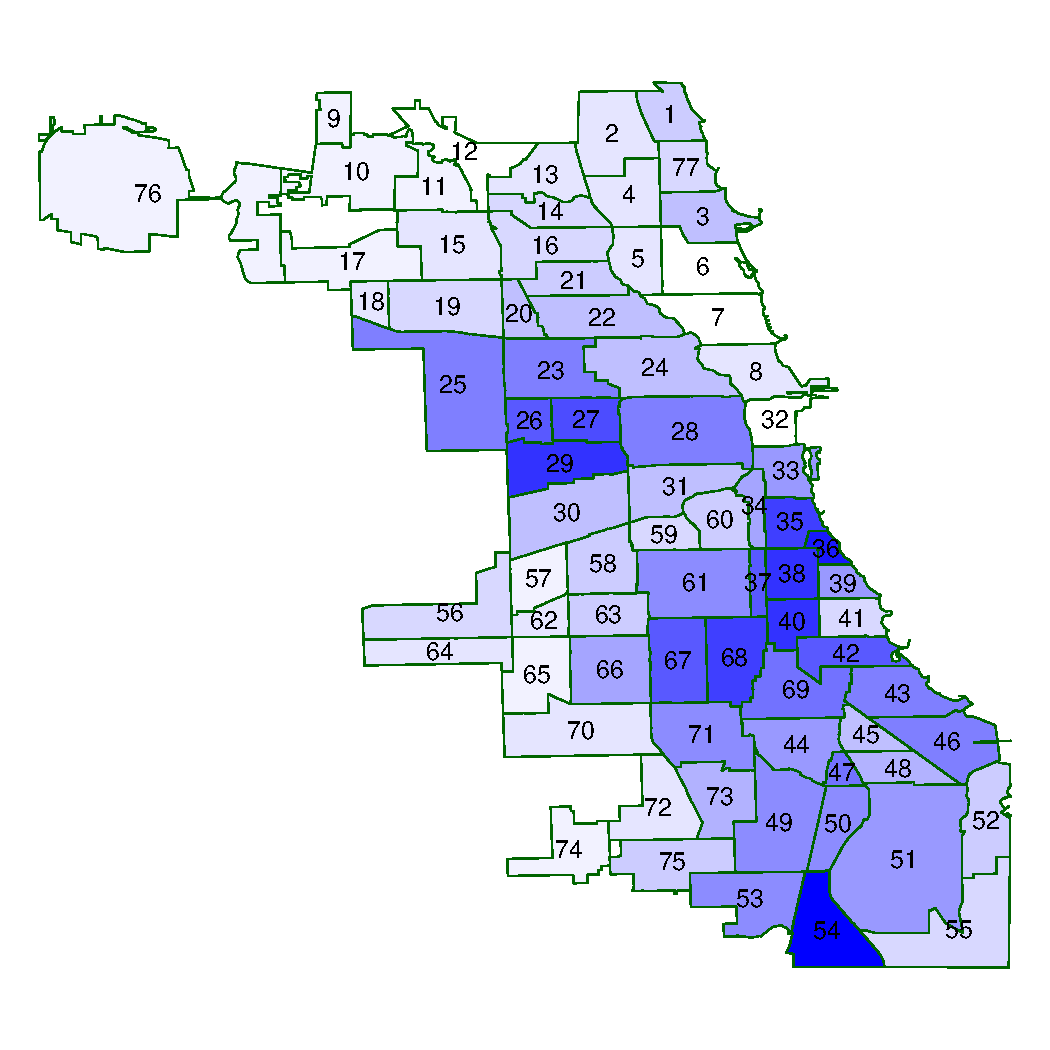
\includegraphics[width=0.45\textwidth]{fig/demo-f4.pdf}}
%\subfigure[Residential stability]{\includegraphics[width=0.22\textwidth]{fig/demo-f5.pdf}}
\subfigure[Ethnic diversity]{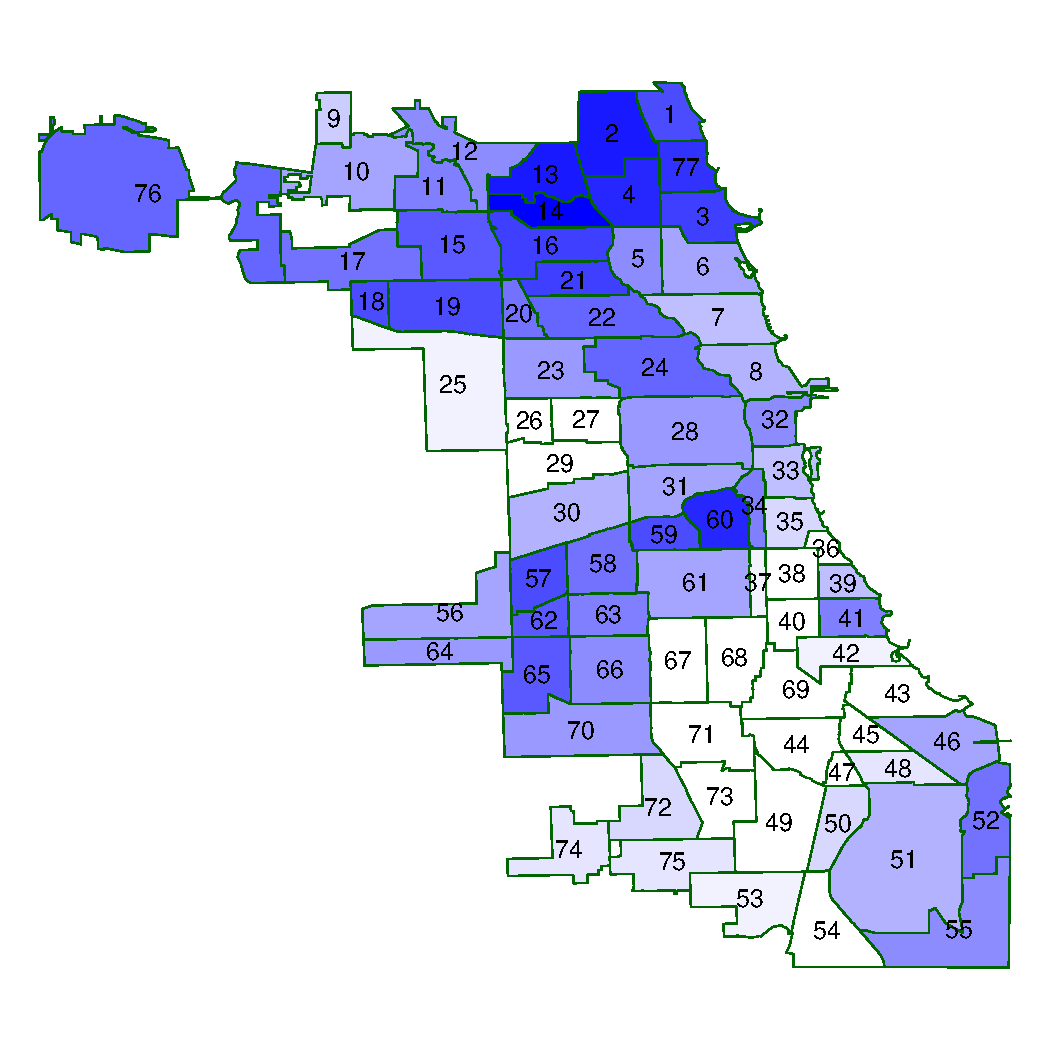
\includegraphics[width=0.45\textwidth]{fig/demo-f6.pdf}}
%\subfigure[Percentage black]{\includegraphics[width=0.22\textwidth]{fig/demo-f7.pdf}}
%\subfigure[Percentage Hispanic]{\includegraphics[width=0.2\textwidth]{fig/demo-f8.pdf}}
%\subfigure[\textred{Percentage white}]{\includegraphics[width=0.2\textwidth]{fig/demo-f8.pdf}}
\caption{(a)-(d) Demographics in Chicago by community areas. Darker colors indicate higher values. Each demographic feature is normalized into $[0,1]$.}
\label{fig:demo-f}
\end{figure*}





\subsection{Nodal Feature: Demographics}

Socioeconomic and demographic features of neighborhoods have been
widely used to predict crime~\cite{Bogo14, HsPu93, WoMe12, SaHi07}. Previous studies have shown that crime rate correlates with certain demographics. For example, \cite{Jac61, GrSa09} suggests that population diversity leads to less crime in certain neighborhoods. 
In our study, we include demographic information from the US Census Bureau's Decennial Census ~\cite{census-data}.   Using 2010 census information would overlap with the time in which crime is measured. Instead, we use year 2000 demographic data because we are interested in predictors that precede temporally the period in which crime rates are evaluated. The demographics include the following features:

\textsf{total population, population density, poverty, disadvantage index, residential stability, ethnic diversity, race distribution}.


The poverty index measures the proportion of community area residents
with income below the poverty level. The disadvantage index is
a composite scale based on prior work \cite{SRE97}, a function of 
poverty, unemployment rate, proportions of families with public
assistance income, and proportion of female headed households. 
 The residential stability measures home ownership and proportion of
residents who lived in the neighborhood for more than one year. Racial
and ethnic diversity is an index of heterogeneity~\cite{GrSa09} based on six
population groups, including: Hispanics, non-Hispanic Blacks, Whites,
Asians, Pacific Islanders and others.


Figure~\ref{fig:demo-f} visualizes the crime rate and demographics features in Chicago by community areas. Comparing with Figure~\ref{fig:crime-ca}, it is clear that the crime rate and poverty index and disadvantage index are consistent,  the ethnic diversity shows an inverse correlation, and the total population has little correlation with crime.



Table~\ref{tb:demo} shows the Pearson correlation coefficient between various demographics features and the crime rate at community area level. The corresponding p-value is also calculated and shown in the table to indicate the significance of the correlation coefficient.  There  are in total $77$  community areas in Chicago. Table~\ref{tb:demo} shows such correlation with several most correlated features. We can see that the poverty index and disadvantage index positively and strongly correlate with crime, while the ethnic diversity negatively correlates with crime. Other features such as total population, population density, and residential stability  have weaker correlations. One counter-intuitive observation is that the total population has a weak and negative correlation with crime. The reason is that we use crime rate in each community area, which is already normalized by the population, and therefore the total population and population density have less impact. 


\begin{table}[h]
\vspace{-5mm}
\centering
\caption{Pearson correlation between demographic features  and crime rate (\textbf{*} indicates significant correlations with p-value less than $5\%$). }
\begin{tabular}{|c||c|c|}
\hline
Feature & Correlation & p-value \\ \hline \hline
Total Population & -0.1269 &  0.2716 \\ \hline
Population Density & -0.1972  & 0.0855 \\ \hline
Poverty Index & \textbf{0.5573*} & 1.403e-07 \\ \hline
Disadvantage Index & \textbf{0.5959*} & 1.082e-08 \\ \hline
Residential Stability  & -0.0453 &  0.6965 \\ \hline
Ethnic Diversity & \textbf{-0.5545*} &  1.678e-07 \\ \hline
Percentage of Black & \textbf{0.6696*} &  2.779e-11 \\ \hline
Percentage of Hispanic  & \textbf{-0.3820*} &  0.0006 \\ \hline
\end{tabular}
\label{tb:demo}

\end{table}

\nop{
\begin{table}[h]
\centering
\caption{Demographic feature description and correlation with crime.}
\vspace{-5mm}
\begin{tabular}{|l|l|r|r|}
\hline
Abbr. & Description & Pearson & p-value \\ \hline
TP & total population & -0.1269 &  0.2716 \\ \hline
PD & population density & -0.1972  & 0.0855 \\ \hline
PI & poverty index & 0.5573 & 1.403e-07 \\ \hline
DI & disadvantage index & 0.5959 & 1.082e-08 \\ \hline
RS & residential stability  & -0.0453 &  0.6965 \\ \hline
ED & ethnic diversity & -0.5545 &  1.678e-07 \\ \hline
PB & percentage of Black & 0.6696 &  2.779e-11 \\ \hline
PH & percentage of Hispanic  & -0.3820 &  0.0006 \\ \hline
\end{tabular}
\label{tb:demo}
\end{table}
}


\subsection{Nodal Feature: Point-of-Interest (POI)}

While demographics are traditional census data, POI is a type of  modern data that provide fine-grained information about locations. We collect POI from FourSquare~\cite{poi-data}. POI data from FourSquare provide the venue information including venue name, category, number of check-ins, and number of unique visitors. We mainly use the major category information because categories can characterize the neighborhood functions. There are 10 major categories defined by FourSquare:

\textsf{food, residence, travel, arts \& entertainment, outdoors \& recreation, college \& education, nightlife, professional, shops, and event.}


\begin{figure}[tb]
\centering
%\subfigure[Food]{\includegraphics[width=0.2\textwidth]{fig/poi-dist1.pdf}}
\subfigure[Nightlife]{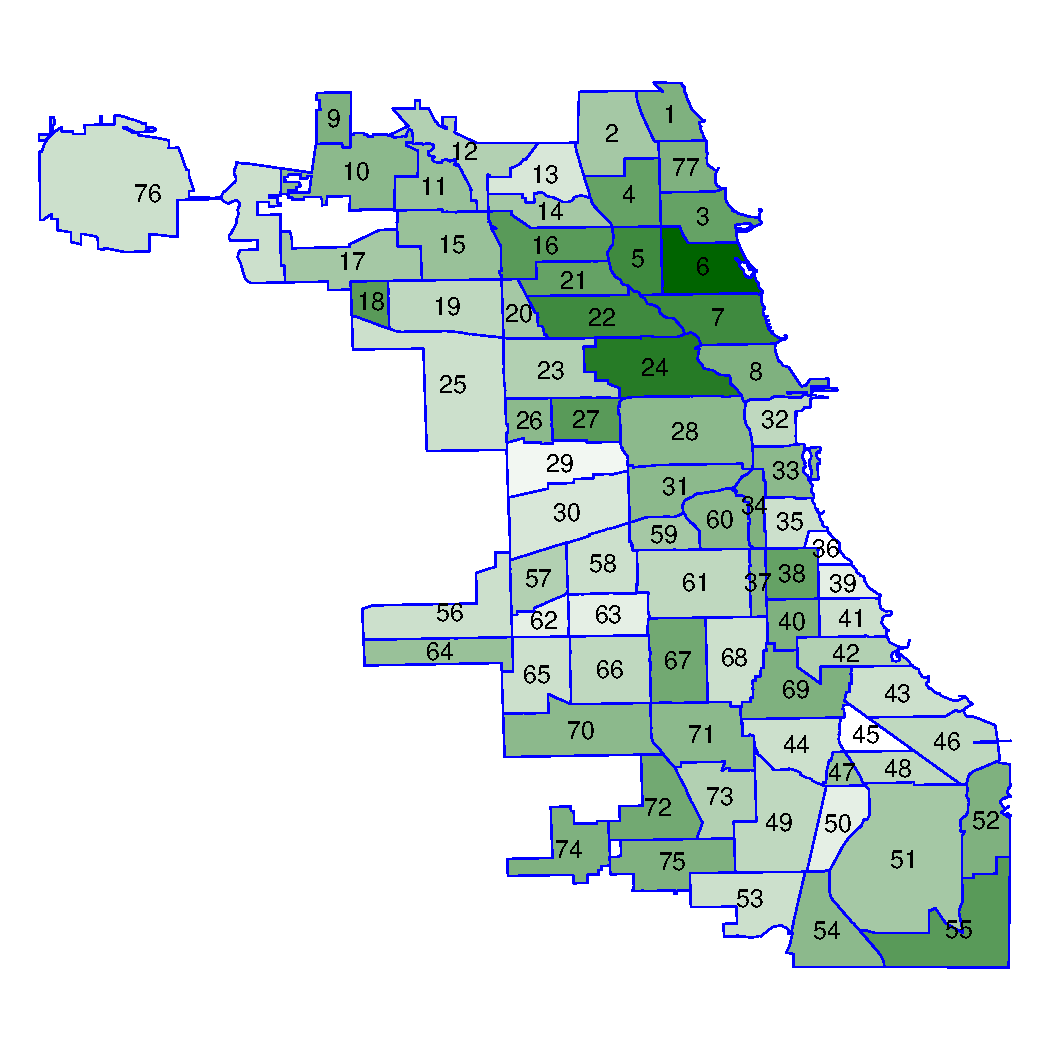
\includegraphics[width=0.45\textwidth]{fig/poi-dist7.pdf}}
%\subfigure[Travel]{\includegraphics[width=0.2\textwidth]{fig/poi-dist3.pdf}}
\subfigure[Professional]{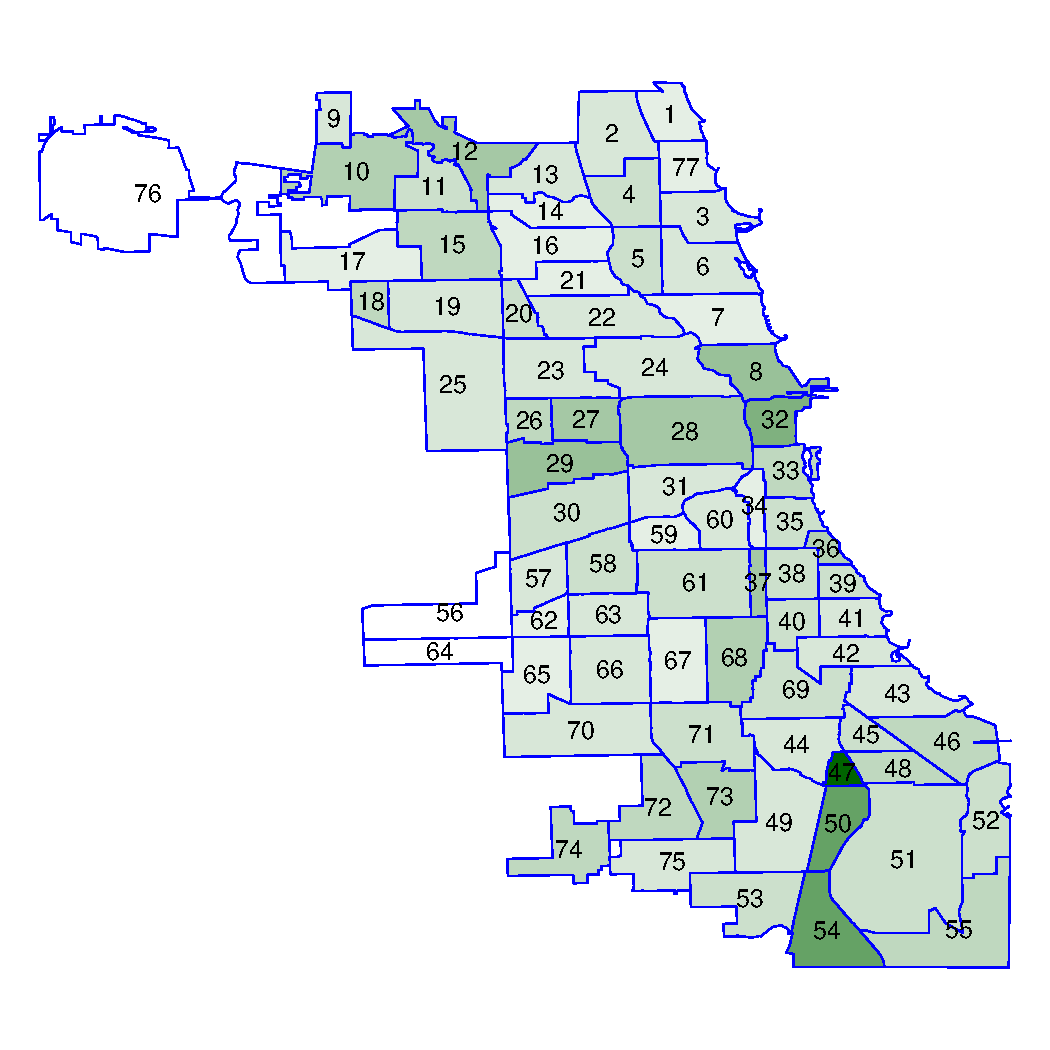
\includegraphics[width=0.45\textwidth]{fig/poi-dist8.pdf}}
%\subfigure[Shops]{\includegraphics[width=0.2\textwidth]{fig/poi-dist9.pdf}}
\caption{POI ratio per neighborhood. The saturation of color is proportional to the ratio value. The ``professional'' category distribution is more consistent with the crime distribution, and therefore it is the most correlated with crime. Meanwhile, the ``nightlife'' category is negatively correlated with Chicago crime. The POI ratios are independently normalized for different POI categories.}
\label{fig:poi-coef}
\end{figure}

In total, we have crawled \num{112000}  POIs from FourSquare for Chicago. Most of these POIs are in the downtown area of Chicago. For the purpose of visualization, we normalize the POIs count per category by the total POI count in a neighborhood and plot two selected categories, i.e. nightlife and professional, in Figure~\ref{fig:poi-coef}.  The darker colored neighborhoods in Figure~\ref{fig:poi-coef} are the ones with a higher proportion of residence POIs.



\begin{table}[h]
\centering
\caption{Pearson correlation between POI category and crime rate (\textbf{*} indicates significant correlations with p-value less than $5\%$).}
\vspace{2mm}

\label{tb:poi-corr}
\begin{tabular}{|c ||c|c|}
\hline
POI category & Correlation & p-value \\ \hline \hline
Food & -0.1543 &  0.1803 \\ \hline
Residence &  -0.0610 &  0.5984 \\ \hline
Travel & -0.0017 &  0.9883 \\ \hline
Arts \& Entertainment & -0.0049 &  0.9661 \\ \hline
Outdoors \& Recreation &  0.0668 &  0.5637 \\ \hline
College \& Education & -0.0078 &  0.9473 \\ \hline
Nightlife &  -0.1553 &  0.1775 \\ \hline
Professional & \textbf{0.3221*} &  0.0043 \\ \hline
Shops & -0.1676 &  0.1450 \\ \hline
Event & 0.2196 &  0.0549  \\ \hline
\end{tabular}
\end{table}



In Table~\ref{tb:poi-corr} we show the Pearson correlation between POI category and crime rate. The category ``professional''  is most significantly correlated with the crime rate. Under the professional POI category, there are some venues with a large population concentration, such as transportation center, convention center, community center, and coworking space. In those venues, the  population volume is high and residential stability is low, therefore the professional POI counts positively correlates with crime rate.  One counter-intuitive observation is that ``nightlife'' category is not positively correlated with crime ($-0.1553$). This can be seen in Figure~\ref{fig:poi-coef}(a). The majority of nightlife venues in Chicago are located in the northern area, while most crime incidents occur in the downtown area.



\subsection{Edge: Geographical Influence}

Together with the US census demographics data, we also collected the boundary shape files of Chicago, which are used to calculate the geographical influence feature.
Previous studies have also shown that the crime rate at one location is highly correlated with nearby locations~\cite{GSGL01, Bur88}. Such geographical influence is also frequently used in the literature~\cite{ACC00, MoSa97}. It is calculated as:
\begin{equation}
\vec{F^g} = W^g \cdot \vec{Y},
\label{eq:spatial}
\end{equation}
where $W^g$ is the spatial weight matrix. If region $i$ and $j$ are not geospatially adjacent, $w_{ij}^g = 0$; otherwise, $w_{ij}^g \propto distance(i,j)^{-1}$.

\begin{figure}[t!]
\centering
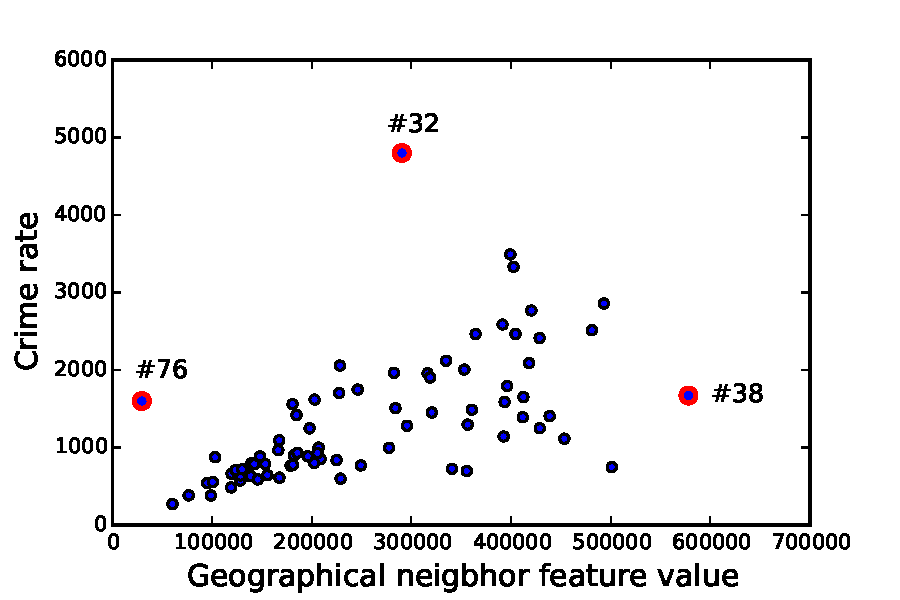
\includegraphics[width=0.8\textwidth]{fig/spatial-crime-rate.pdf}
\caption{The correlation between geographical influence feature  and crime rate. In the plot we marked out three outliers and their corresponding community area ID.}
\label{fig:spatial}
\end{figure}

In Figure~\ref{fig:spatial},  we plot crime rate with respect to geographical influence calculated in Eq.~\ref{eq:spatial}. We observe an obvious positive correlation, which means if nearby neighborhoods have a high crime rate, the focal neighborhood is more likely to have a high crime rate. We also do observe a few outliers in Figure~\ref{fig:spatial}. These neighborhoods show different crime rate in their nearby neighborhoods compared to their own. For example, as we can also see in Figure~\ref{fig:crime-ca}, community area \#38 locates in an area where the the neighbors have high crime rates but its crime rate is relatively low; in contrast, neighborhood \#32 has a high crime rate even though its neighbors have relatively low crime. The community area \#76 home of the O'Hare International Airport is far from most of other community areas, however its own crime rate is relative high.



\subsection{Edge: Hyperlinks by Taxi Flow}

In our Chicago taxi dataset, there are \num{1048576} taxi trips in total from October to December in 2013. For each trip, the following information are available: pickup/dropoff time, pickup/dropoff location, operation time, and total amount paid. We requested the taxi trip records from Chicago under the Illinois Freedom of Information Act.  Figure~\ref{fig:taxi-flow} shows a visualization of the major flows at community level.

\begin{figure}[htb]
\centering
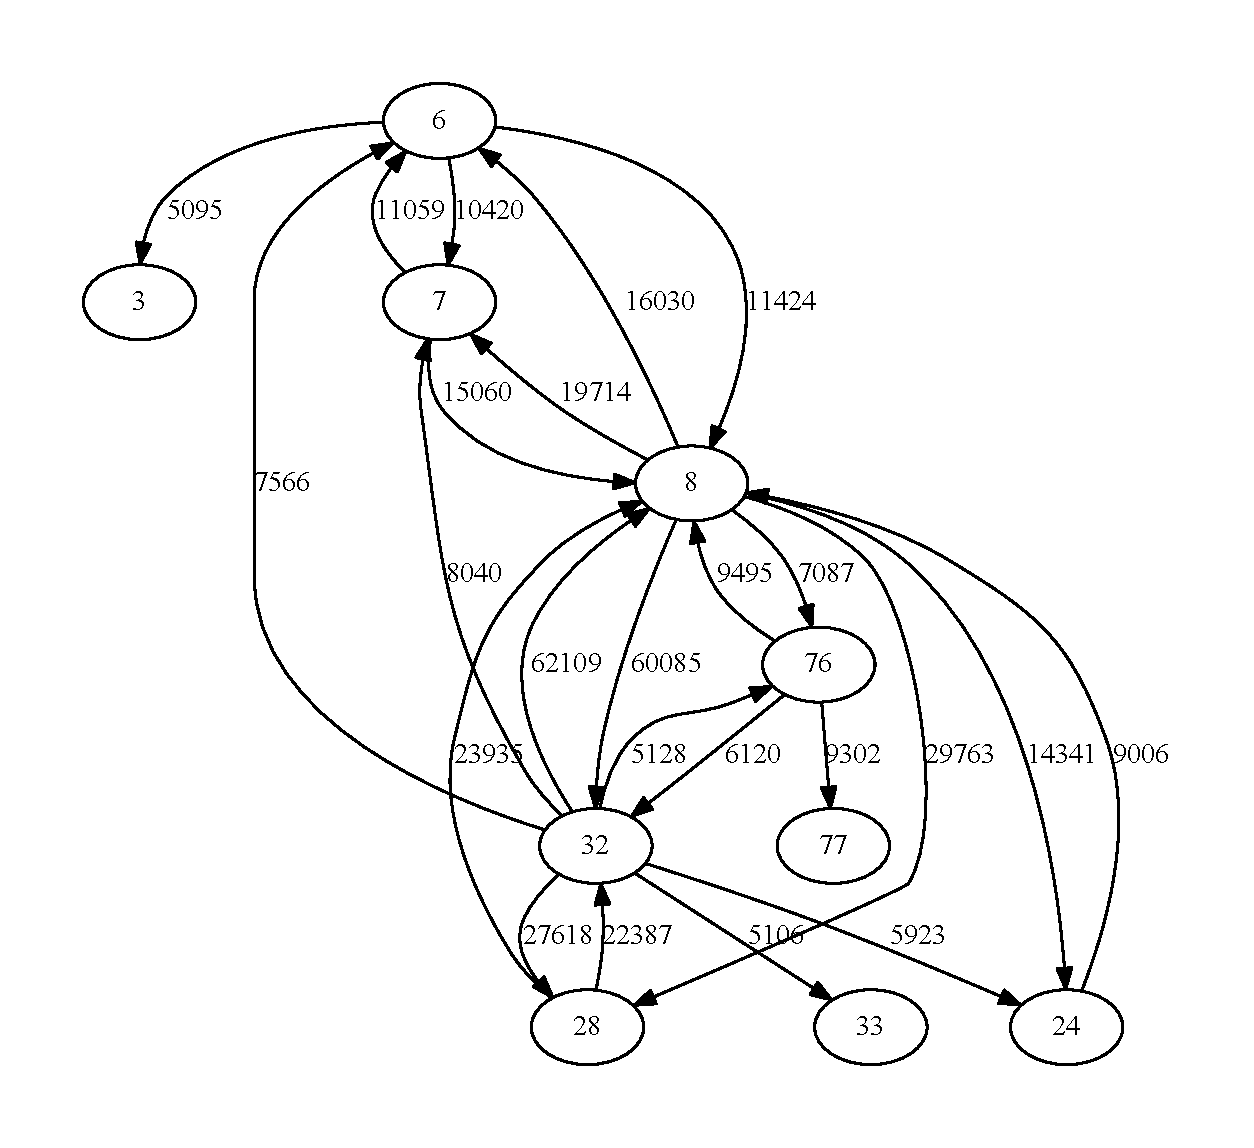
\includegraphics[width=0.7\textwidth]{fig/taxiflow.pdf}
\caption{Major taxi flows between neighborhoods. The label on the edge shows the count of taxi trips  commuting between two community areas from October to December months in 2013. We set a threshold (more than 5,000 trips) on the flow and only plot high volume flows. The label on a node is the ID of its corresponding community area. We can see that there are several hub community areas, such as \#6, \#8, \#32, which are all in the downtown areas. }
\label{fig:taxi-flow}
\end{figure}


One of our hypotheses is that the social interaction among two community areas propagates crime from one region to another.
The Chicago taxi data captures the social interactions among various community areas. To calculate this, we first map all taxi trips to community areas to get the taxi flow $w_{ij}\ \forall i,j \in \{1, 2, \cdots n\}$. Then the taxi flow lag is constructed by the product of social flow and the crime rate of neighboring regions as follows
\begin{equation}
\vec{F^t} = W^t \cdot \vec{Y}.
\label{eq:taxi}
\end{equation}
The taxi flow $W^t$ is a matrix with entry $w_{ij}$ denoting the taxi flow from $i$ to $j$. Note that $\forall i$, $w^s_{ii} = 0$ in matrix $W^t$, because we have to exclude the crime in the focal area from its own predictor. The semantic of this taxi flow feature is how much crime in the focal area is contributed by its neighboring areas through social interaction.

The correlation between taxi flow and crime rate is shown in Figure~\ref{fig:taxi-corr}. From the scatter plot, we can see that overall the crime rate is positively correlated with the taxi flow. There are two  outliers clearly shown in Figure~\ref{fig:taxi-corr}. The community area \#32 is the downtown Loop, which has the highest crime rate and is hard to predict by taxi flow. Another anomalous community area (\#47) has relatively low crime rate by itself. However, this area has a lot of in flows from high-crime communities. 




\begin{figure}[ht]
\centering
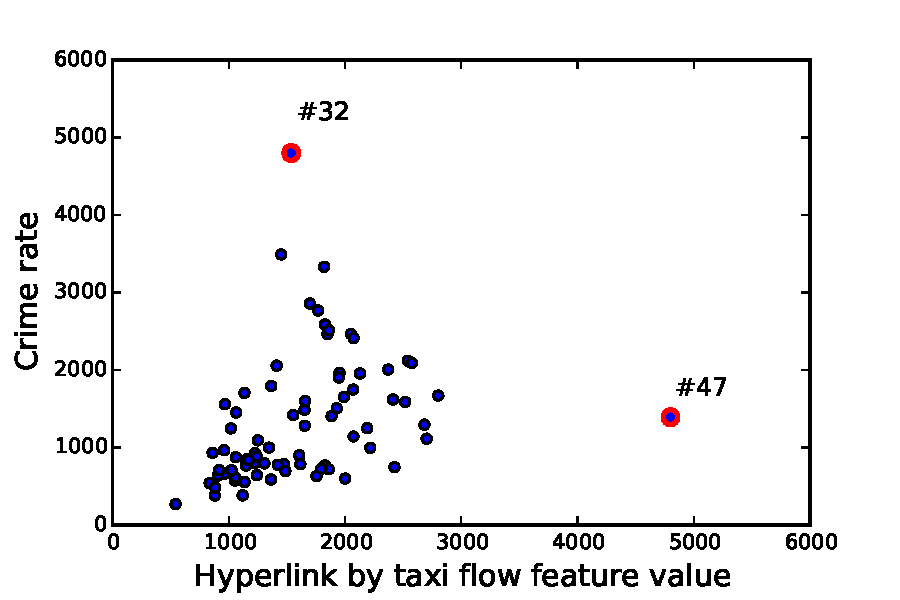
\includegraphics[width=0.8\textwidth]{fig/taxi-flow-percent.pdf}
\caption{Correlation between taxi flow feature and crime rate. In the plot, we marked out two outliers and their corresponding community area ID.}
\label{fig:taxi-corr}
\end{figure}



%%%%
\nop{
\begin{figure}[t]
\centering
\subfigure[Arts POI w.r.t. crime count]{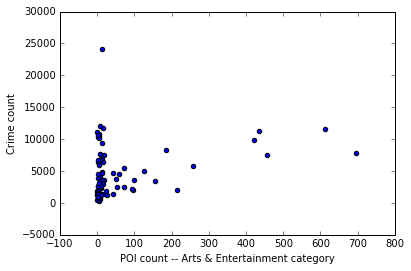
\includegraphics[width=0.23\textwidth]{fig/poi-arts.png}}
\subfigure[Arts POI w.r.t. crime rate]{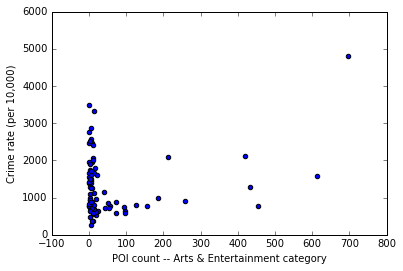
\includegraphics[width=0.23\textwidth]{fig/poi-arts-crimeRate.png}}
\caption{Comparison between the correlation of arts POI category count w.r.t. crime count and crime rate. The crime rate is crime count normalized per 10,000 population. \textred{draw fitted line, show $R^2$ error}}
\label{fig:demo-extra}
\end{figure}
}

\nop{
It is widely believed that the two geospatially close neighborhoods have higher interactions, and thus the crime rate is similar. 


In Table~\ref{tb:spatf}, the correlations between spatial flow and crime count are presented. Overall, the geographical influence is positively correlated with the crime count. At community area level, the geographical influence has a Pearson correlation coefficient of $0.4415$ with the actual crime count. In the crime prediction setting, the various communities have different areas and number of residents. In order to make fair comparison and eliminate the population effects, it is reasonable to compare the spatial flow against crime rate, namely the crime count per 10,000 population. In the second setting, we show the result of using crime rate, and there is a significant increase in the correlation.

At tract level, the spatial flow correlation with crime is reduced, as shown in the third and fourth row of Table~\ref{tb:spatf}. The reason is that tract is a relatively small geographical area, which is usually populated by $4,000$ people\footnote{Census Tract \url{http://www.census.gov/geo/reference/gtc/gtc_ct.html}}. The crimes are usually not commuted too close to the affenders' home.  

\begin{table}[h!]
\caption{Correlation between geographical neighbor feature and crime count.}
\label{tb:spatf}
\centering
\begin{tabular}{|l|r|}
\hline
Settings & correlation \\ \hline
CA level, crime count  & 0.4415 \\ \hline
CA level, crime rate per 10,000 population & 0.5969 \\ \hline
Tract level, crime count with social flow & 0.2377 \\ \hline
Tract level, crime rate per 10,000 population & 0.0771 \footnote{Census data is not 2010}\\ \hline
\end{tabular}
\end{table}



\begin{table}[h!]
\caption{Correlation between social flow and crime count.}
\label{tb:lehd}
\centering
\begin{tabular}{|l|r|}
\hline
Settings & correlation \\ \hline
CA level, crime count & 0.2072 \\ \hline
CA level, crime count, weighted social flow & 0.3217 \\ \hline
CA level, crime rate per 10,000 population & 0.5898 \\ \hline
CA level, crime rate, weighted social flow & 0.6014 \\ \hline
Tract level, crime count & 0.4462 \\ \hline
Tract level, crime rate per 10,000 population & 0.1306 \footnote{Census data is not 2010}\\ \hline
\end{tabular}
\end{table}



Table~\ref{tb:taxi} shows the correlation between taxi flow feature and crime. Under different settings, the taxi flow keep a positive correlation with the crime.


\begin{table}[h]
\caption{The correlation between taxi flow and crime}
\label{tb:taxi}
\begin{tabular}{|l|r|}
\hline
Settings & Correlation Coefficient \\\hline
Taxi flow count, crime rate & 0.2337 \\ \hline
Taxi flow count, crime count & 0.2514 \\ \hline
Taxi flow percentage, crime rate & 0.3315 \\ \hline
Taxi flow percentage, crime count & 0.3418 \\ \hline
\end{tabular}
\end{table}


}






